\documentclass[11pt,a4paper,oneside]{article}


\usepackage[nodayofweek,level]{datetime}
\usepackage[margin=15mm]{geometry}
\usepackage{amsmath}
\usepackage{hyperref}
\usepackage{amsthm}
\usepackage{amssymb}
\usepackage{tikz-cd}
\usetikzlibrary{calc}
\usepackage[greek,british]{babel}
\usepackage{float}
\usepackage{wrapfig}
\usepackage{caption}
\usepackage{subcaption}
\usepackage[toc,page]{appendix}
\usepackage{color}
%\usepackage[utf8]{inputenc}
\usepackage{mathrsfs}
\usepackage[square]{natbib}

%\usepackage[T1]{fontenc}
\usepackage{inconsolata}

\usepackage{fancyvrb}
\usepackage{listings}
\definecolor{ltblue}{rgb}{0,0.4,0.4}
\definecolor{dkblue}{rgb}{0,0.1,0.6}
\definecolor{dkgreen}{rgb}{0,0.4,0}
\definecolor{dkviolet}{rgb}{0.3,0,0.5}
\definecolor{dkred}{rgb}{0.5,0,0}
\usepackage{lsthaskell}

%\lstset{fancyvrb=true,basicstyle=\sffamily,columns=flexible}

%\lstset{language=Haskell}


\setlength{\parindent}{0em}
\setlength{\parskip}{1em}



\hypersetup{
	colorlinks=true,
	linkcolor=blue,
	citecolor=blue,
	filecolor=black,
	menucolor=black,
	urlcolor=blue	
}


\title {RRB-Trees: Efficient Concatenation of Immutable Vectors}
\author {Elias Khoury}

\begin{document}

\maketitle

\textit{
Vectors are a common datastructure used in everyday programming to represent an indexed sequence of data. Depending on the implementation, a vector datastructure can be optimised for certain operations. The purpose of this report is to present an implementation for a general purpose datastructure which performs well across all possible use cases. This is achieved by using a balanced tree structure to store the elements of the vector in the leaves of the tree. The focus will be mainly on the concatenation operation of the vector, and the methods used in order to ensure that modifying the structure of the tree to accommodate more elements does not effect the runtime of other operations. 
}

\pagebreak

\tableofcontents

\pagebreak


\section{Typical Uses}

In a typical programming situation, it can often be difficult to estimate what datastructure to use for a problem, a good example is a cons list which is present as the default implementation for a List datastructure in Haskell. For smallscale applications this method has many advantages for pattern matching purposes, but the O(n) access of elements dramatically slows down programs for largescale uses, in which case a Vector may be a better choice. In specialised scenarios this choice may be a blessing to a developer looking for specific use cases, however a case can also be made for an all-rounder solution which can be used in a variety of non specific scenarios. RRB-Vectors designed to be an ideal solution for such non specialised problems.  This makes it a perfect addition to a standard library for programming languages, the original paper by \cite{bagwell2011rrb} outlines the goal of imtegrating the final product into the Scala 14 programming language, meanwhile a ready to use implementation for Closure is available online\citep{marczyk2012clojure}.


RRB-Trees are a purely functional datastructure, and with that property comes a great advantage. Since purity can be guaranteed for the various manipulations of the datastructure, the operations lend themselves well to being parallelised. This can be efficiently be done by delegating parts of the tree structure to computations in various threads without worrying about interference. Bulk operations come very handy in the field of dynamically generated text\citep{blelloch1990vector}. Sever side generation of HTML code can now efficiently be done for multiple users at a time by essentially filling out a HTML template with a user's specific data. Dynamically generating HTML code is something that as websites have become more complicated, is now much more of a challenge\citep{hull2006balancing}. Likewise serverside database querying benefits from such a datastructure due to the fact that basic queries can be stored on file and simply built up dynamically to suit the needs of the current operation. This will greatly increase the output on high load servers which are required to both generate queries are runtime, and also perform bulk updates on existing queries in order to serve a specific user. There are even tools being developed which use high speed query generation in order to prevent SQL injections by dynamically generating legitimate queries and using those to check for attacks\citep{halfond2006}.


\section{Overview of the Datastructure}

In this implementation, Vectors are represented using a tree structure, with each leaf being an element in the sequence. Indexing is done by traversing the tree in order to reach the desired leaf node, concatenation is done by taking two trees and joining them into a new tree containing the leaves from both trees. With that in mind it is important to make sure that the speed of the concatenation operation should not impact the accessibility of the leaves since that will negatively impact the speed of other operations. 

\begin{figure}[h]
	\centering
	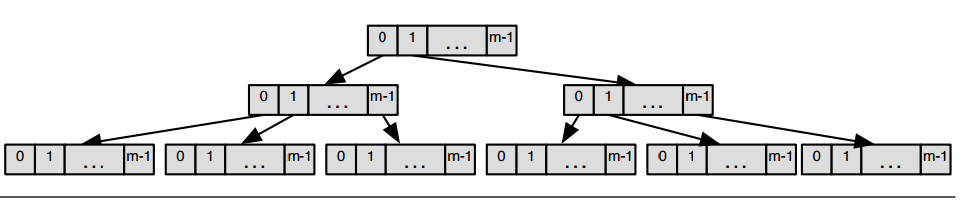
\includegraphics[scale=0.5]{img/radixbalancedtree.png}
	\caption{A balanced tree of branching factor 4\citep{bagwell2011rrb}}
\end{figure}

Indexing into the tree structure relies on the method of a radix search\citep{angle1999radix}. For a balanced tree with branching factor m, it is possible to calculate the number of leaf nodes at each level (l) using the formula:
 $\lfloor i / (m^l) \rfloor\  \%\  m$.
The search operation functions by descending the tree and choosing subtree which will contain the desired leaf node. An example of these calculations for the example tree above where m is 4 and the height is 2 is as follows:
\begin{center}
\begin{tabular}{l | l}
(1). $\lfloor 5 / (4^{2}) \rfloor = 0$ & (3a). $ \lfloor 5 / (4^{0}) \rfloor = 5 $ \\
(2). $\lfloor 5 / (4^{1}) \rfloor = 1$ & (3b). $ 5 \quad \% \quad 4 = 1 $ \\ 
\end{tabular}
\end{center}

\begin{figure}[h]
	\centering
	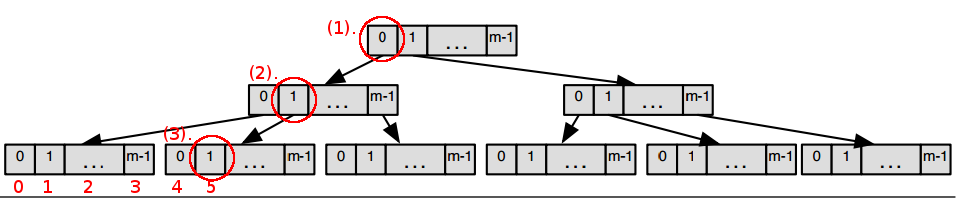
\includegraphics[scale=0.5]{img/radixbalancedtree_search.png}
	\caption{Searching the tree for index 5}
\end{figure}

Each result of the calculation is the subtree at every level that needs to be explored. The disadvantage of this implementation is that it relies on each branch having exactly a branching factor of m. This restriction makes other operations on the tree more difficult, take for example the concatenation operation. For a tree with a constant branching factor, appending elements from another tree would require a linear copy of all the leaves in the second tree to the first. In fact, in order to find a solution which allows a less than linear time concatenation, it is necessary to relax the branching factor in order to allow some flexibility in the data structure.  

The method used to relax the data structure is similar to methods found in 2-3-Trees or Finger trees\citep{okasaki1996purely}. The idea is to have a variable branching factor which allows the data structure to be manipulated in a way to accomodate more elements. In the analysis section the impact this decision has on performance will be discussed. The main important aspect is that a variable branching factor breaks the method of a radix search, it is now impossible to determine the numbers of leaves in each node. As such, alternative methods need to be discussed, however the final solution still relies heavily on the core principles behind radix search.


\subsection{Main Features}

The main features are the most basic vector operations to illustrate the key components of the datastructure. 

\begin{center}

\begin{tabular}{| l | l |}
\hline
Operation & Description\\
\hline
Index & Indexes into the vector\\
Concat & Joins two vectors into a single vector\\
head   & gets the first element in the vector\\
tail   & removes the first element in the vector\\
init  & removes the last element in the vector\\
last   & get the last element in the vector\\
\hline
\end{tabular}

\end{center}

\section{Analysis of Runtime}

\begin{wrapfigure}{r}{0.3\textwidth}
	\centering
	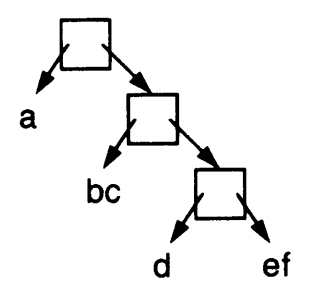
\includegraphics[scale=0.5]{img/ropes.png}
	\caption{Ropes Data Structure}
\end{wrapfigure}

The task of concatenating two trees can be done in a multitude of ways. However, how the tree is structured can restrict which methods can be applied. For example, given two trees with a constant branching factor, the only way to get a perfect concatenation of the trees is to do a linear copy of each element into a new tree. Likewise, if speed is the only concern then an O(1) solution is possible by simply making a new root and joining that to the two new trees, this is similar to a concept used in ropes\citep{boehm1995ropes}. For this application both solutions have their disadvantages, firstly a linear cost is far too slow for large scale applications, however simply making a new root each time is dangerous because after multiple concatenations the tree will simply degenerate into a linked list. This will negatively impact other operations like indexing as they will become constant time. The balance that needs to be struck is a method which is fast, but doesn't degenerate the data structure.

\subsection{Relaxed Radix Structure}

The relaxed radix structure is a variant of the Radix tree which allows for the possibility of nodes not being full. As such, the height is no longer bounded by log(n) like in a typical balanced tree, but by an additional invariant based on the minimum and maximum branching factor\citep{bagwell2011rrb}. Given two branching factors: $b_{min}, b_{max}$, the height of the tree is bounded by the two branching factors. The heights can be expressed as:
\begin{gather*}
h_{max} = log_{b_{min}} N \quad h_{min} = log_{b_{max}} N \\
alternatively, \\
h_{max} = \frac{1}{log_{b_{min}}}lg N \quad h_{min} = \frac{1}{log_{b_{max}}}lg N
\end{gather*}
Using these equations for the minimum and maximum heights of the tree, we can calculate the ratio how unbalanced the tree could be based using:
\begin{equation*}
h_r = \frac{lg\ b_{max}}{lg\ b_{min}}
\end{equation*}
A perfectly balanced tree will have a ratio of 1, in this scenario, the chosen values for the branching factors are $m_{max} = m_{min} + 1$, in order to keep the tree as close to perfectly balanced as possible.


Given this new structure, it is no longer possible to calculate how many leaves are in each subtree, since that subtree might be unbalanced. In that case, any unbalanced node needs to have some metadata attached to it indicating how many leaves are in each subtree. This adds a constant time factor to the radix search. The complexity of finding a leaf is now $O(m * Log(n))$ where m is a constant cost associated with an unbalanced node. 

\begin{figure}[h]
	\centering
	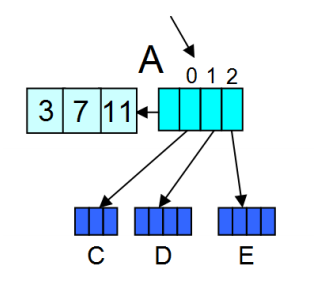
\includegraphics[scale=0.5]{img/sizesmetadata.png}
	\caption{The sizes metadata associated with each unbalanced node\citep{bagwell2011rrb}}
\end{figure}

The invariant introduced is only relevant to operations which manipulate the tree structure. As such, with those operations it is important that there is an effort made to keep the tree structure balanced in order to reduce the constant time cost with indexing.

\subsection{Concatenation}

The concatenation operation starts at the leftmost branch of the right tree and the rightmost branch of the left tree. It takes those two subtrees and creates a new tree containing the leaves from both subtrees. In order to maintain balance, the subtrees are not simply copied, but they are broken down to their respective leaves and then reconstructed. This rebalancing operation tries to first favour a branching size of m over m-1 in order to maintain balance, this has the effect of redistributing the nodes so they fill each branch from left to right.

\begin{figure}[H]
	\centering
	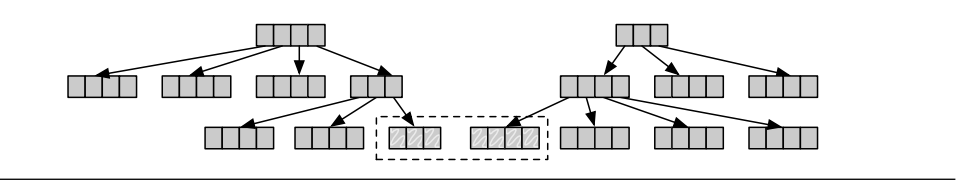
\includegraphics[scale=0.5]{img/concat1.png}
	\caption{The nodes from each subtree that need to be removed\citep{stucki2015rrb}}
\end{figure}

\begin{figure}[H]
	\centering
	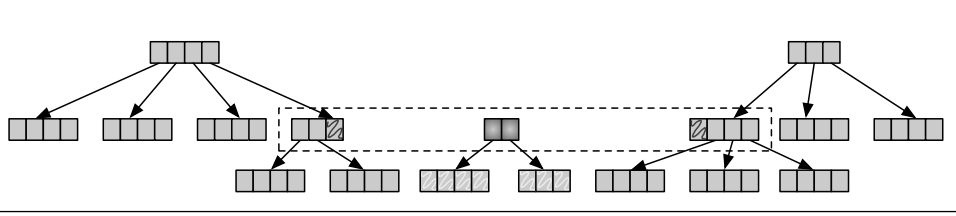
\includegraphics[scale=0.5]{img/concat2.png}
	\caption{Constructing a new tree with the nodes rebalanced\citep{stucki2015rrb}}
\end{figure}

Once this is done, the algorithm moves up the two trees and joins the nodes at each level, each time creating a dummy root of size two which will be deleted in the subsequent iterations. At each level it is important to rebalance the nodes. This is done by taking the children of the nodes being merged and copying them to the new dummy root. Thanks to lazy evaluation and sharing, this copying operation should have little overhead.

\begin{figure}[H]
	\centering
	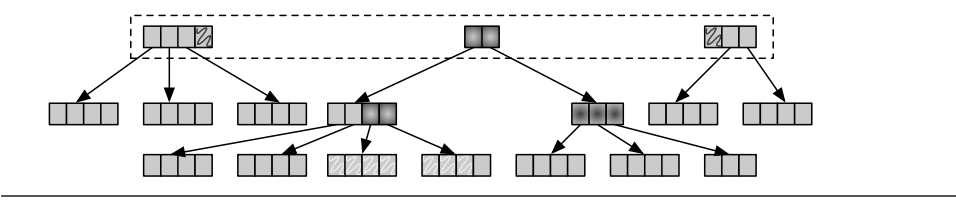
\includegraphics[scale=0.5]{img/concat3.png}
	\caption{Merging the nodes and creating a new dummy node\citep{stucki2015rrb}}
\end{figure}

\begin{figure}[H]
	\centering
	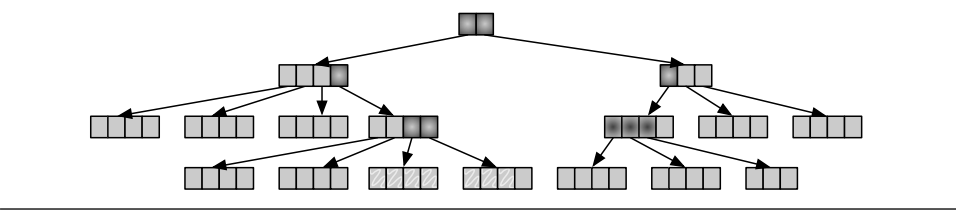
\includegraphics[scale=0.5]{img/concat4.png}
	\caption{The final join of the two trees\citep{stucki2015rrb}}
\end{figure}

The next few diagrams show how the algorithm moves up the tree. This variant of the algorithms is an alteration of the one presented in the original paper\citep{bagwell2011rrb}, \cite{stucki2015rrb} present an alternative method which focuses on the practicality of the datastructure as a whole. In the original paper, the method described did not prioritise each node having exactly m children. Instead, tree balance was the main factor taken into account, which results in trees containing nodes with fewer than m children. Although the method presented in the original paper is several times quicker than the chosen method, it would often result in trees that were very tall, this directly affects the speed of the indexing operations which is bounded by the depth of the tree. Therefore, in order to have a practical, general purpose data structure, it is important to compromise the speed of the concatenation operation in order to not negatively effect the other operations.

\subsection{Branching Factor}

Choosing the branching factor, m is a crucial factor for calculating the runtime of each operation. As stated, accessing leaf nodes requires a full traversal of the tree, for n elements in a perfectly balanced tree the runtime is bounded by $O(log_m n)$. There is a small caveat with a tree structure which allows us to exploit the branching factor in order to make tree traversal trivial. In the two papers presented, a branching factor of 32 was chosen, one good reason is that this allows cache sizes to be exploited since each node can fit perfectly in a cache line\citep{stucki2015rrb} (although this assumes the datastructure itself has no overhead which may not be the case for high level languages). Another reason is that having a high branching factor very large impact on the depth of the tree. With a branching factor of 32, storing 10,000,000 items in the tree will only create a tree of depth 5. In fact, considering the case of indexing into the vector using a 32 bit integer, the maximum value accessible is 4,294,967,296 ($2^{32}$) meaning that if that were the size of the entire vector then the tree would still only be of depth 7. With the assumption that indexing is bounded by a 32 bit integer, any operation which runs in $O(log_m(n)$ is bounded by the maximum depth of the tree which is a constant of 7, effectively making the operation run in constant time\citep{bagwell2011rrb}.

	\begin{center}
	\begin{tabular}{| l || c | c |}
		\hline
		& RRB-Vector & With m = 32 \\
		\hline
		indexing & $ log_m $ & eC\\
		update & $m \times log_m $ & eC \\
		insert ends & $ m \times log_m $ & aC \\
		concat & $ m^2 \times log_m $ & L v.s. eC \\
		split & $ m \times log_m $ & eC \\
		\hline
		\end{tabular}
	\end{center}

Empirical tests have also shown that a branching factor of 32 is also the most ideal. The figure below shows the index and update times for several branching factors, the choice to be made is a trade off between the two operations, the values of m with the best ratios are 8,16,32 meaning they all lead to good solutions, however 32 was chosen simply because it leads to slightly faster index times which is worth the cost of the slower updates.

\begin{figure}[H]
	\centering
	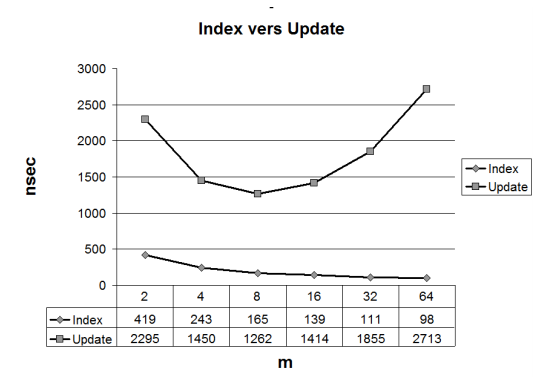
\includegraphics[scale=0.5]{img/indexupdate.png}
	\caption{Index verses update of various branching factors\citep{bagwell2011rrb}}
\end{figure}

\section{Chosen Language}

RRB-Trees are a purely functional data structure, they rely heavily on the concept of sharing and lazy evaluation when copying and manipulating segments of the tree. In order to take advantage of these features, it would be ideal to use a functional language to write the implementation. The concepts behind RRB-Trees emerged from research done on developing Scala and OCaml, as such it would be interesting to compare the difference with an implementation in a similar functional language. 

Haskell makes a good candidate for such a comparison. Like Scala, Haskell is used in a variety of industrial applications, a large one being Facebook\citep{marlow2014haxl}. Haskell is also ideal for translating mathematical concepts into programs since the syntax very closely resembles mathematics, this makes the task of understanding algorithms written in Haskell much easier since they are distilled into bite sized functions which have many parallels in structure to the theory.

\section{Implementation}

\subsection{Tree Structure}

The tree is represented using a Haskell data structure, each node contains its height in the tree, along with a list of its children and the sizes metadata should the node be unbalanced. The leaves themselves contain the elements of the vector, and since leaves are always balanced they have no size metadata. 

\begin{haskell}

branchingFactor :: Int
branchingFactor = 32

type Height = Int
type Sizes = [Int]

data Tree a = Node Height [Tree a] Sizes | Leaf [a]
    deriving (Show)

\end{haskell}

\subsection{Indexing}

Indexing into the tree is performed using the relaxed radix search algorithm. For efficiency, the function alternates to using radix search if it encounters a balanced subtree. How this is done is by pattern matching on the sizes metadata. If there is no metadata then the distribution of leaves in each subtree must be equal. In this case it is possible to calculate which subtree the desired leaf is in using the formula: $\lfloor i / (m^l) \rfloor\  \%\  m$ (where l is the current height of the tree). The function recurses on the desired subtree, In order to do this, a new index needs to be calculated in order to fined the desired leaf relative to that subtree. This new index is the current index minus how many leaves come before this subtree, what is left over is the offset of the desired leaf withing the chosen subtee. The value nodeCount indicates which subtree the desired leaf is in, iOffset then multiplies that with how many leaves are in each subtree in order to calculate the new index for a single subtree.

\begin{haskell}

relaxedSearch :: Int -> Tree a -> a 
relaxedSearch i (Leaf as) = as !! (i `mod` branchingFactor)
relaxedSearch i (Node l ts [])  = relaxedSearch (i - iOffset) (ts !! nodeCount) 
                where nodeCount = (i `div` (branchingFactor ^ l)) `mod` branchingFactor
                      iOffset   = (branchingFactor ^ l) * nodeCount
relaxedSearch i (Node l ts ss)  = relaxedSearch (i - iOffset) (ts !! subTree)
                where iOffset   = if subTree == 0 then 0 else ss !! (subTree - 1) 
                      subTree   = length (takeWhile (< i) ss) 

\end{haskell}

In the case where the node is unbalanced, the sizes metadata needs to be accessed, this keeps a running total of all the leaves in each subtree. Firstly the correct subtree is located by indexing into sizes list until an element is found where the total number of leaves so far exceeds the desired index. The previous value in the sizes list contains the number of leaves that come before the desired subtree, this is used to calculate the new index, and the function recurses on the desired subtree.

\subsection{Getting / Removing elements}

The operations: head,tail,init,last are all operations that require tree traversal to access the leaf elements. Each function is defined using a helper function that gets or removes a child at a certain height. In this case the only elements that need to be manipulated are the first and last elements of the vector, these are always on the 0th level of the tree, the leaf nodes.

\begin{haskell}

head' :: Tree a -> a
head' t = head leaves
    where Leaf leaves = getLeftChild t 0

tail' :: Tree a -> Tree a
tail' t = dropLeftChild t 0

init' :: Tree a -> Tree a
init' t = dropRightChild t 0

last' :: Tree a -> a
last' t = last leaves
    where Leaf leaves = getRightChild t 0

\end{haskell}

Starting with the getLeftChild, getRightChild function, they are both defined in terms of a function called getEndChild, which when fed a certain input will either go down left subtrees, or right subtrees. 

\begin{haskell}

getEndChild :: Tree a -> Int -> ([Tree a] -> Tree a) -> Tree a
getEndChild (Leaf a) _ _       = Leaf a
getEndChild (Node l [] ss) n f = Node l [] ss
getEndChild (Node l ts ss) n f | l == n    = Node l ts ss
                               | otherwise = getEndChild (f ts) n f

\end{haskell}

The getEndChild function pattern matches on each level of a node, if it encounters a node which is at the height that it is looking for, it returns that node. Otherwise it keeps descending down that node's children. The third input of this function is a function that given a list of trees will return a single tree, this allows the getEndChild function to be customised to descend down a node based on a criteria. For the getLeftChild and getRightChild functions the functions supplied are head and last, these always pick the first or last tree in a list which is always the left or right subtree.


Deleting a subtree is similar. The dropLeftChild function descends down a tree, and if it reaches the level where a subtree needs to be deleted then it returns an empty node. If not it simply recurses down the leftmost branch. The dropRightChild is simply a mirror of this function, in the interest of space only the former is shown

\begin{haskell}

dropLeftChild :: Tree a -> Int -> Tree a
dropLeftChild (Leaf as) _      = Leaf (tail as)
dropLeftChild (Node l [] _) _ = Node l [] []
dropLeftChild (Node l ts _) n | l == n = Node l [] []
                              | otherwise = Node l ([dropLeftChild (head ts) n] + + tail ts) []

\end{haskell}

\subsection{Concatenation}

The concatenation function begins by merging the leftmost branch of the right tree with the rightmost branch of the left tree into a new tree of height two. The leaves are redistributed to ensure that the left branch of the new tree is full. if there are not enough leaves to fill both branches, then the tree is unbalanced and the sizes need to be calculated and stored.

\begin{haskell}

mergeEnds :: Tree a -> Tree a -> Tree a
mergeEnds t1 t2 = Node 2 [Node 1 leftChild [], Node 1 rightChild []] (if lSize == rSize then [] else [lSize,rSize])
        where Node _ leftLeaves _  = getRightChild t1 1
              Node _ rightLeaves _ = getLeftChild t2 1
              leaves        = leftLeaves + + rightLeaves
              leftChild     = take branchingFactor leaves
              rightChild    = drop branchingFactor leaves
              [lSize,rSize] = map (length.stripLeaf) [last leftChild,last rightChild]
              stripLeaf     = \ (Leaf a) -> a

\end{haskell}

A similar method is done for the subsequent heights. At each level of the merge process, the mergeAt function is called. This takes the appropriate subtrees from the left and right tree for some arbitrary height n, and merges them into the new tree. The merge process is done my the mergeRebalance function, since this implementation of RRB-Trees favours branches with branching factor m, when copying nodes from the left and right tree into the middle of the tree, they need to be rebalanced in order to redistribute the nodes to maintain the branching factor. Therefore at each level this has to be done.

\begin{haskell}

mergeAt :: Int -> (Tree a,Tree a,Tree a) -> (Tree a,Tree a,Tree a)
mergeAt n (t1,t2,t3) = (leftTree,mid,rightTree)
                where leftTree   = dropRightChild t1 n
                      leftChild  = getRightChild t1 n
                      mid        = mergeRebalance (leftChild,t2,rightChild)
                      rightTree  = dropLeftChild t3 n
                      rightChild = getLeftChild t3 n

\end{haskell}

The nodes from all three trees need to be merged in a way that maintains the balance of the tree. In order to do this, each node is replaced by its children, and those children are replaced by their children. Then the parent nodes are reconstructed in a way where each new parent is now full with the exception of possibly the last parent. At this stage the sizes metadata needs to also be recalculated using the computeSizes function, this function simply identifies if any nodes are unbalanced and stores a running total of how many leaves are in each subtree.  

\begin{haskell}

mergeNodes :: [Tree a] -> [Tree a]
mergeNodes ns = case firstMerge of
                  []                 -> []
                  ((Leaf _):ns)      -> balanceLeaves secondMerge
                  ((Node l _ _):ns)  -> map (\ts -> Node l ts (computeSizes ts l)) (collect branchingFactor secondMerge)
                where firstMerge  = concat (map getKids ns)
                      secondMerge = concat (map getKids firstMerge)

\end{haskell}

The mergeRebalance function takes the three trees that need to be merged and merges them using the mergedNodes function. It then creates a dummy node with two children containing the output of mergedNodes.  

\begin{haskell}

mergeRebalance :: (Tree a,Tree a,Tree a) -> Tree a
mergeRebalance (t1,t2,t3) = Node (l + 1) [left,right] (computeSizes [left,right] (l+1))
                    where mergedNodes = mergeNodes[t1,t2,t3]
                          Node l _ _  = t1
                          leftChildren = (take branchingFactor mergedNodes)
                          rightChildren = (drop branchingFactor mergedNodes)
                          left = Node l leftChildren (computeSizes leftChildren l)
                          right = Node l rightChildren (computeSizes rightChildren l)

\end{haskell}

The whole algorithm is tied together by the mergeAt function. Given an input of a particular height of a tree, the mergeAt function will firstly remove the appropriate branches at that level from the left and right tree. It will then take those branches that were removed and feed them into the mergeRebalance function, along with the current state of the middle tree. The result is a new version of the middle tree with the branches merged correctly. By calling the mergeAt function for each level of the trees that are being merged, the middle tree will slowly be built up until it contains all leaf nodes from both trees. This is finally shown using the rrbConcat function, which kickstarts the merge operation by merging the first two extreme nodes to create the middle tree, then feeds the three trees into the mergeAt function.

\begin{haskell}

mergeAt :: Int -> (Tree a,Tree a,Tree a) -> (Tree a,Tree a,Tree a)
mergeAt n (t1,t2,t3) = (leftTree,mid,rightTree)
                where leftTree   = dropRightChild t1 n
                      leftChild  = getRightChild t1 n
                      mid        = mergeRebalance (leftChild,t2,rightChild)
                      rightTree  = dropLeftChild t3 n
                      rightChild = getLeftChild t3 n
                      
rrbConcat :: Tree a -> Tree a -> Tree a
rrbConcat t1@(Node l1 _ _) t2@(Node l2 _ _) = head ts
        where maxHeight = max l1 l2
              left      = dropRightChild t1 1
              middle    = mergeEnds t1 t2
              right     = dropLeftChild t2 1
              (_,Node _ ts _,_) = rrbConcat' maxHeight 2 (left,middle,right)

rrbConcat' :: Int -> Int -> (Tree a, Tree a, Tree a) -> (Tree a, Tree a, Tree a)
rrbConcat' maxl l ts = case maxl == l of 
                       True  -> newTrees
                       False -> rrbConcat' maxl (l+1) newTrees
                    where newTrees = mergeAt l ts

\end{haskell}

\pagebreak

\section{Empirical Evaluation}

The datastructure was evaluated using 189 files which in total contained 382,502,785 characters obtained from the United States Government\citep{obama2014complaints}. Each of the files contained the source code for an HTML table, the objective was to simulate the dynamic generation of HTML code by concatenating each file to append rows at the bottom of the table. The tests were done by keeping a current tree of the HTML code in memory and constantly appending new data to the tree in order to accumulate the HTML code. Once the whole tree was built, the leaf nodes were sequentially written to a file. The runtime of each concatenation operation is shown below, it is worth noting that it took longer to convert the raw HTML code into the Haskell tree structure than it did to actually append the trees together, this is quite a limitation on usability of this data structure. The tests were run using Haskell's clock functions which are not available on the university computers, the version submitted has omitted all the timing functionality, however a full version exits on github\footnote{https://github.com/EliasKhoury/RRB-Trees-in-Haskell}

\begin{figure}[H]
	\centering
	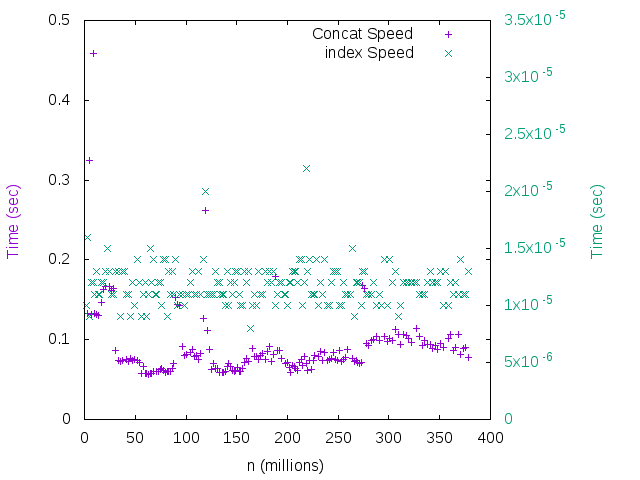
\includegraphics[scale=0.75]{img/analysis.png}
	\caption{analysis of runtime for \~380,000,000 elements}
\end{figure}

As predicted by the mathematical analysis, each concatenation operation seems to run in roughly the same time. For a tree of size 380,000,000 the final tree structure should have only been of height 6. Therefore, despite starting with roughly 16 million elements and ending up with 380 million, the upwards trend for time complexity is ever so slight. Another factor which was measured was the index time, after each concatenation the time taken to index to a random leaf using relaxed radix search was measured. The results show that the index time was far more varied than the concatenation time, it is possible that this is simply down to the balance of the tree, and the operations which took longer time were due to the linear lookup of branches.


One more aspect which required analysis is the effect of the branching factor on the algorithm. The previous tests were run again on a smaller samplesize of about 100,000,000 elements. The performance of the algorithm with branching factors 4.8.16.32.64 are shown below. The axis have been omitted to make the graphs large enough to be readable, however the scale is the same as the previous graph.

\begin{figure}[H]
    \centering
    \begin{subfigure}[b]{0.3\textwidth}
        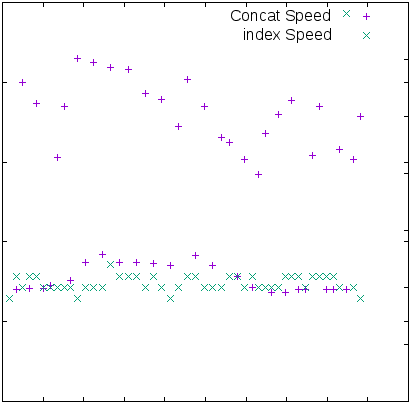
\includegraphics[width=\textwidth]{img/plot4.png}
        \caption{m = 4}
    \end{subfigure}
    ~ %add desired spacing between images, e. g. ~, \quad, \qquad, \hfill etc. 
      %(or a blank line to force the subfigure onto a new line)
    \begin{subfigure}[b]{0.3\textwidth}
        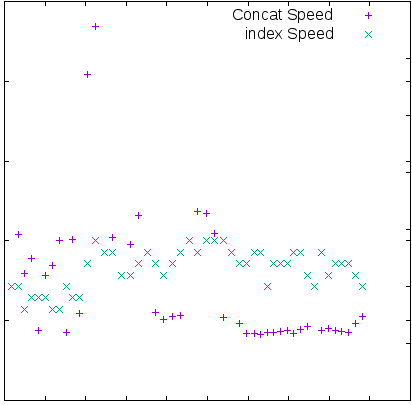
\includegraphics[width=\textwidth]{img/plot8.png}
        \caption{m = 8}
    \end{subfigure}
    \begin{subfigure}[b]{0.3\textwidth}
        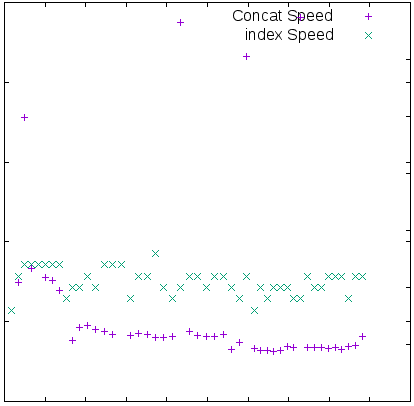
\includegraphics[width=\textwidth]{img/plot16.png}
        \caption{m = 16}
    \end{subfigure}
    
    \begin{subfigure}[b]{0.3\textwidth}
        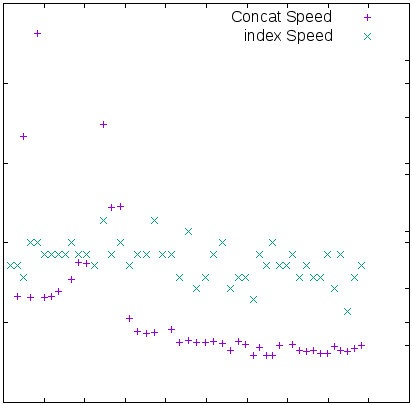
\includegraphics[width=\textwidth]{img/plot32.png}
        \caption{m = 32}
    \end{subfigure}
    \begin{subfigure}[b]{0.3\textwidth}
        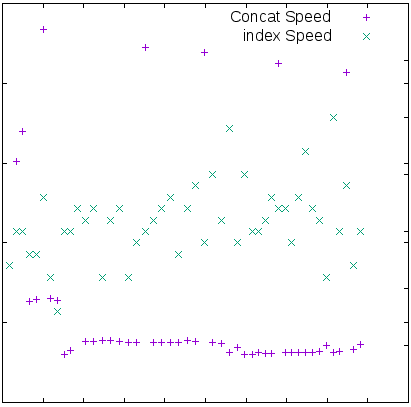
\includegraphics[width=\textwidth]{img/plot64.png}
        \caption{m = 64}
    \end{subfigure}
    ~ %add desired spacing between images, e. g. ~, \quad, \qquad, \hfill etc. 
    %(or a blank line to force the subfigure onto a new line)
\end{figure}

The results of the Haskell implementation seem to mimic the figures shown previously from the work done by \cite{bagwell2011rrb}. The two extremes exhibit the full effects of the branching factor, a branching factor of 4 has by far the slowest concatenation times, this is due to the fact that for 100,000,000 items the tree height will be roughly 14 therefore there will be a lot of rebalancing operations per concatenation. Surprisingly however, the branching factor of 64 exhibits the slowest indexing speeds, this could mainly be down to the linear lookup associated with the relaxed radix search. Since each unbalanced node has a size metadata of length 64, it would take a significant amount of time to search for the desired subtree.

\pagebreak

\bibliographystyle{abbrvnat}
\bibliography{/home/elias/Documents/G52AAD/RRB-Trees/data/report/references}


\end{document}

